\documentclass[12pt,a4paper]{style}

%%%%%%%%% Preamble

% used for figures:
\usepackage{subfigure,graphicx}
% math fonts etc.:
\usepackage{amsmath,amsfonts,amsthm,latexsym,amssymb}
\usepackage{pdfpages}

\usepackage{hyperref}
\hypersetup{
    colorlinks,
    citecolor=black,
    filecolor=black,
    linkcolor=blue,
    urlcolor=black
}
\graphicspath{ {figures/} }
%%%%%%%%%%

\title{\Large \bf
	Austo automobile case study. % proposal title goes here
}

\begin{document}
\tableofcontents
\listoffigures
\newpage
\begin{center}
\Large {\bf{Austo automobile case study}}    
\end{center}

	\section{Context}
	Austo Motor Company is a leading car manufacturer specializing in SUV, Sedan, and Hatchback models. In its recent board meeting, concerns were raised by the members on the efficiency of the marketing campaign currently being used. The board decides to rope in an analytics professional to improve the existing campaign. They want to analyze the data to get a fair idea about the demand of customers which will help them in enhancing their customer experience.
	
	\section{Dataset}
	\begin{figure}[h]
		\centering
		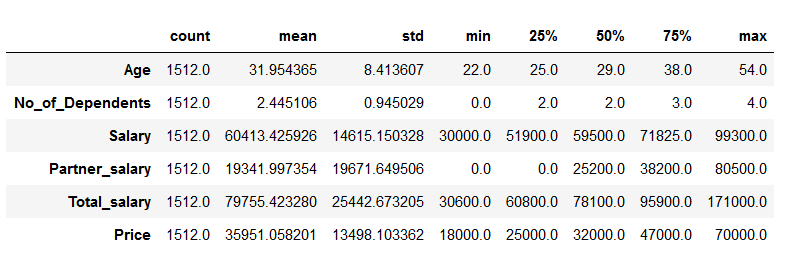
\includegraphics[width=10cm]{stat_summary.png}
		\caption{Statistical summary of numerical variables}
	\end{figure}
	\begin{figure}[h]
		\centering
		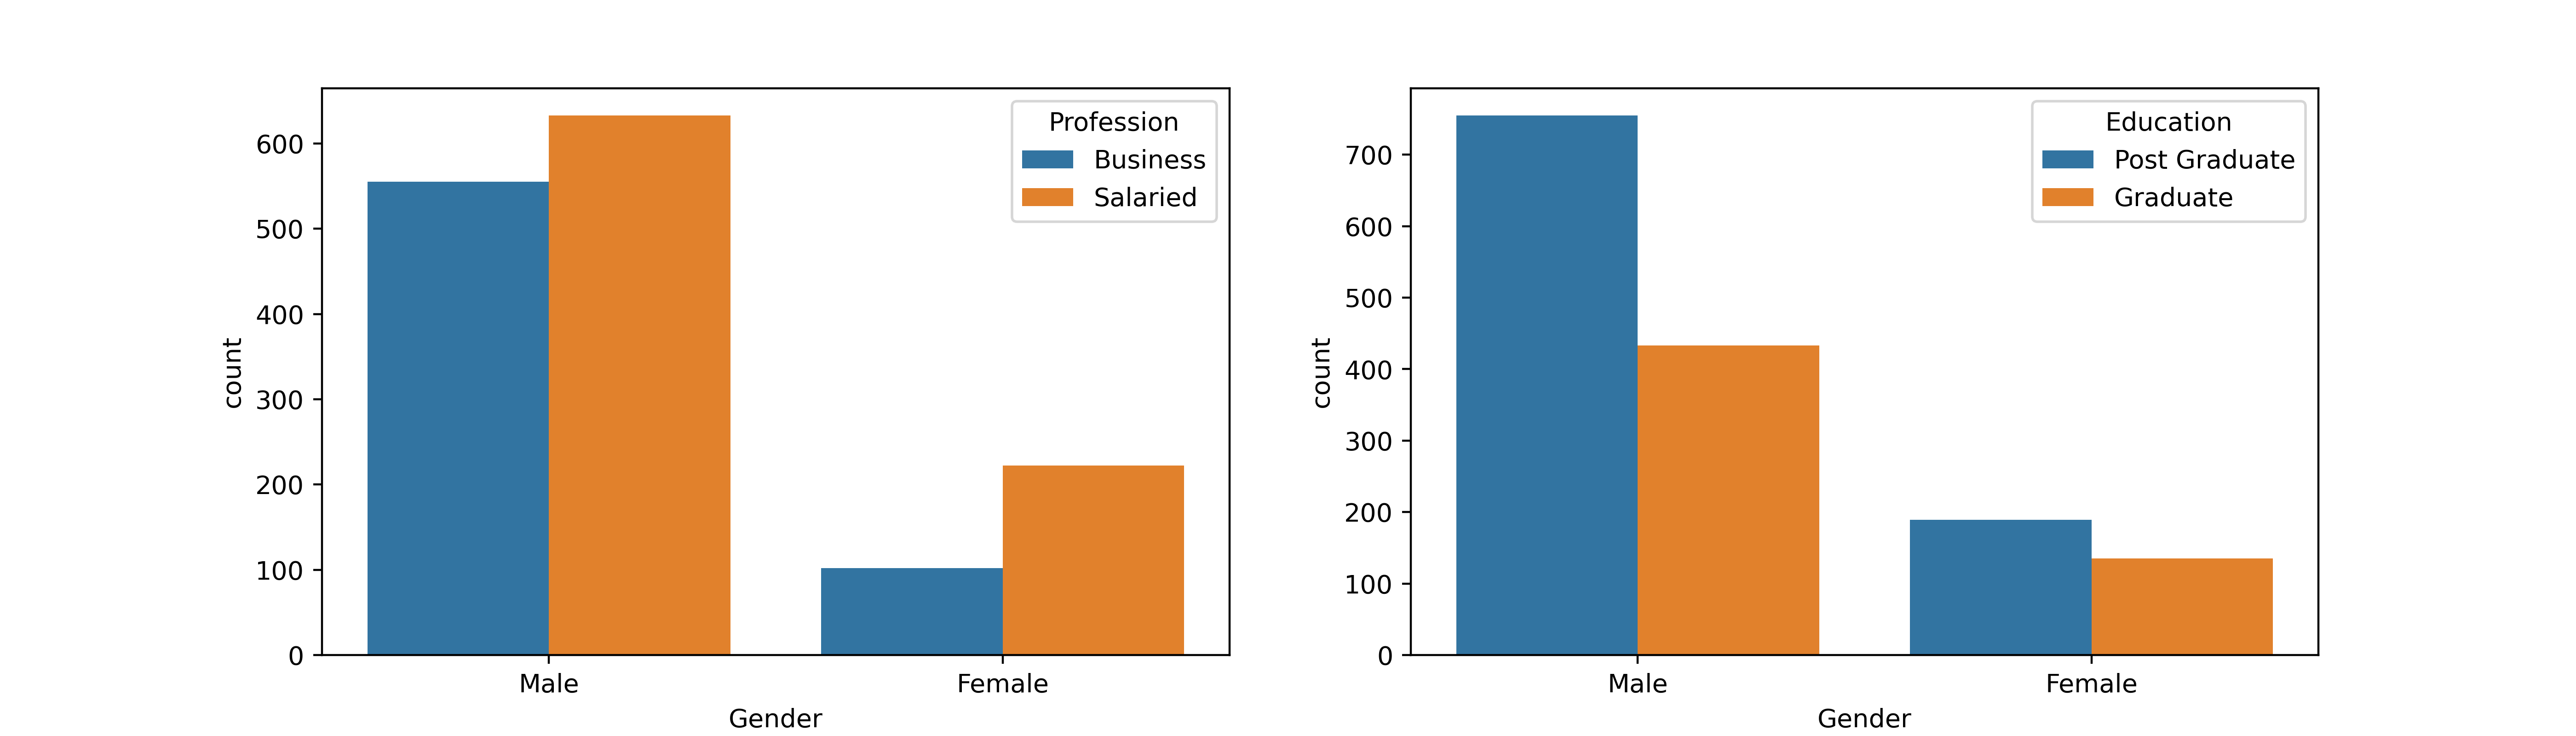
\includegraphics[width=13cm]{about_buyers.png}
		\caption{Gender and Education}
	\end{figure}
	\begin{figure}[h]
		\centering
		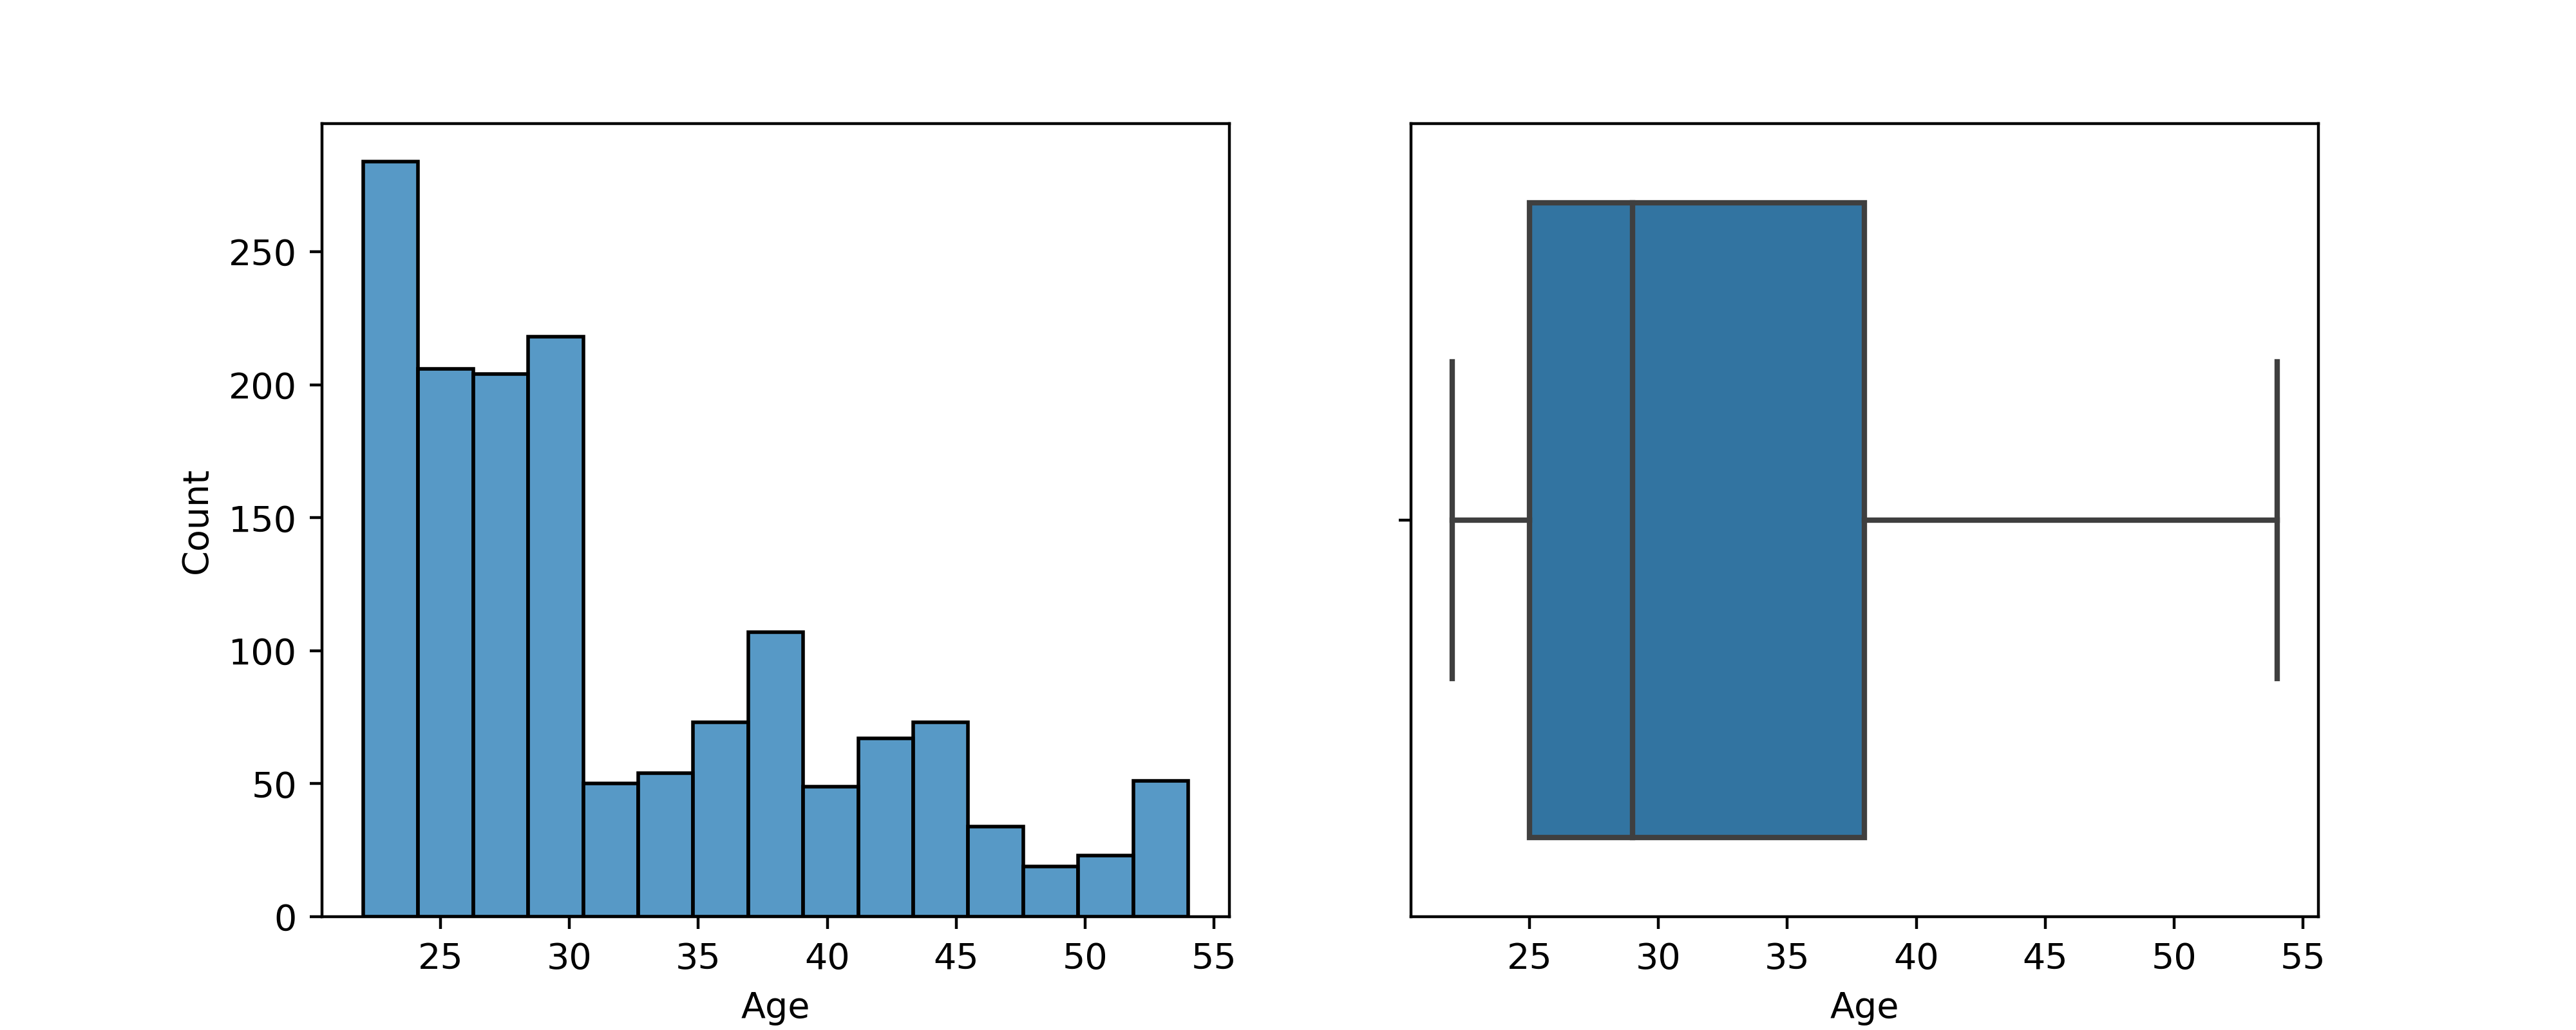
\includegraphics[width=12cm]{Age_dist.png}
		\caption{Age distribution}
	\end{figure}
	\begin{figure}[h]
		\centering
		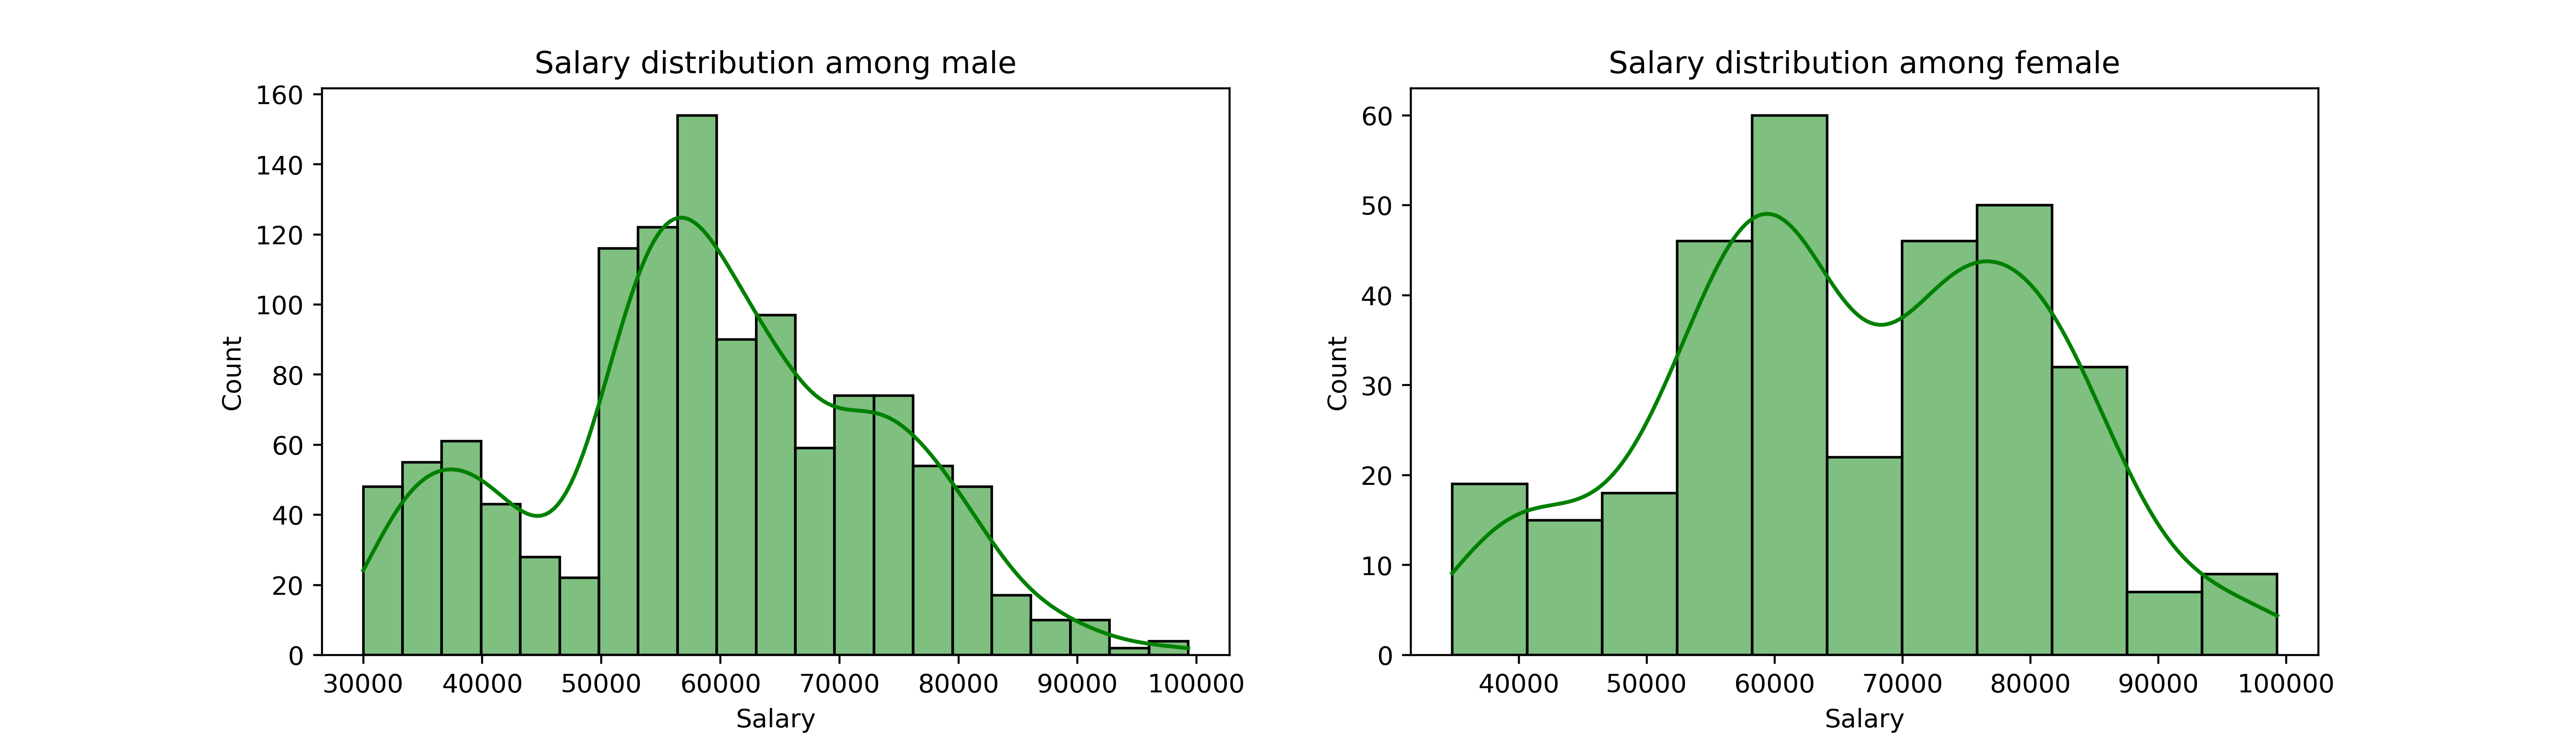
\includegraphics[width=13cm]{salary_gender_dist.png}
		\caption{Salary distribution}
	\end{figure}
	\begin{figure}
		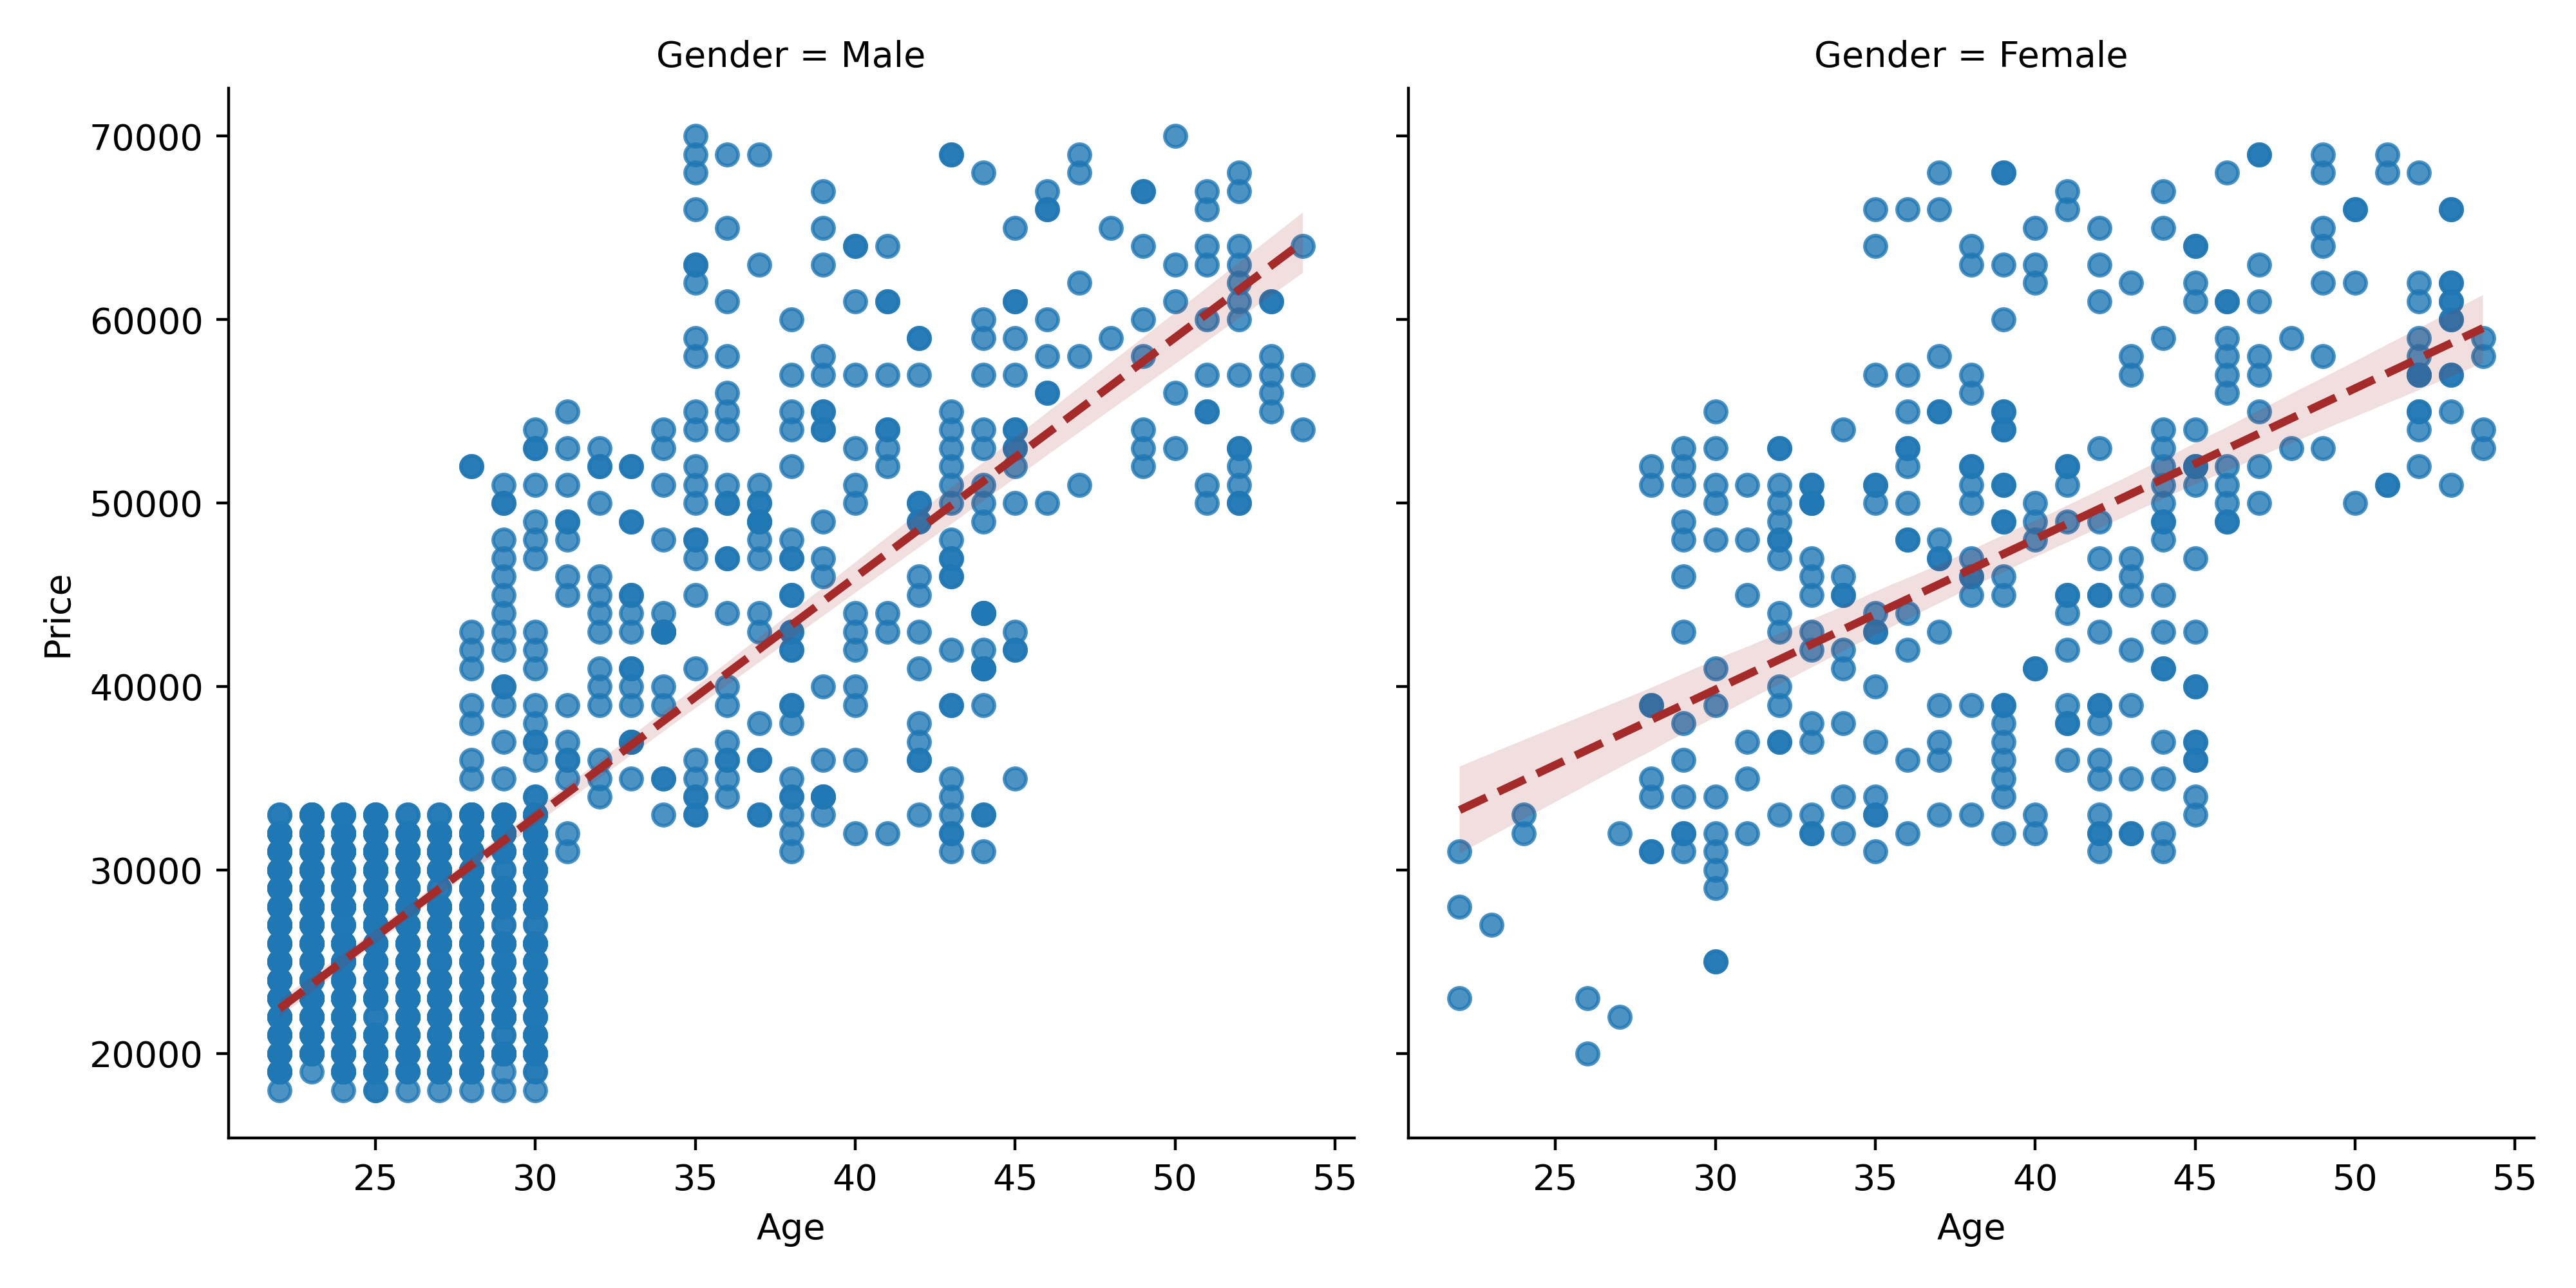
\includegraphics[width=0.55\textwidth]{Age_vs_price.png}
		\caption{Age vs purchase price}
	\end{figure}
    \section{Business Questions}
    \subsection{Preference of SUV among men and women}
		\begin{figure}[h]
			\centering
			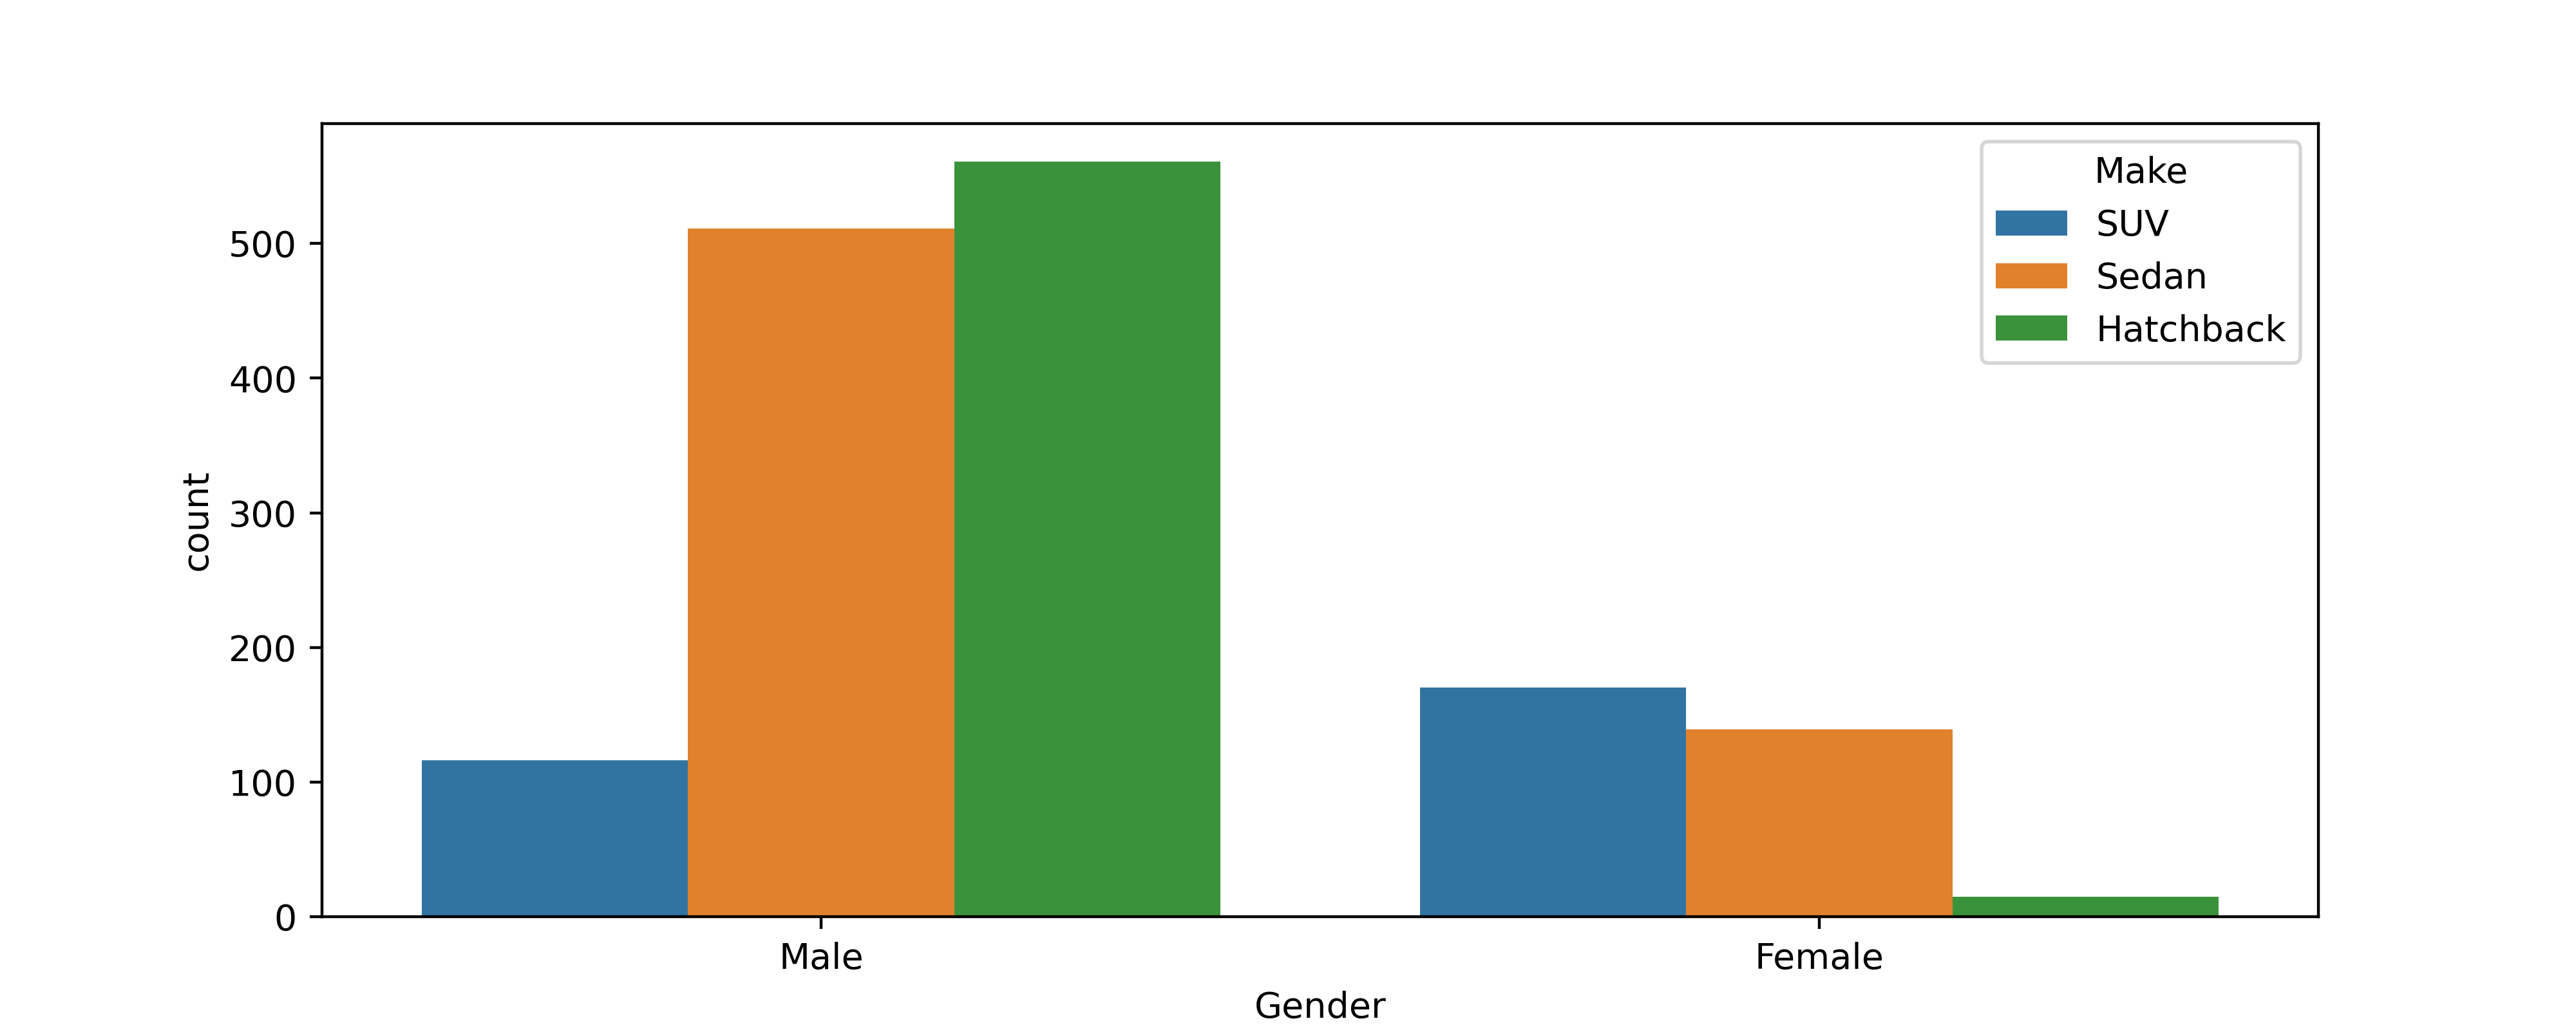
\includegraphics[width=13cm]{make_type_gender.png}
			\caption{Vehicle make preference among male and female}
	\end{figure}
	
    \subsection{Likelihood of a salaried person buying a Sedan}
	\begin{figure}[h]
		\centering
		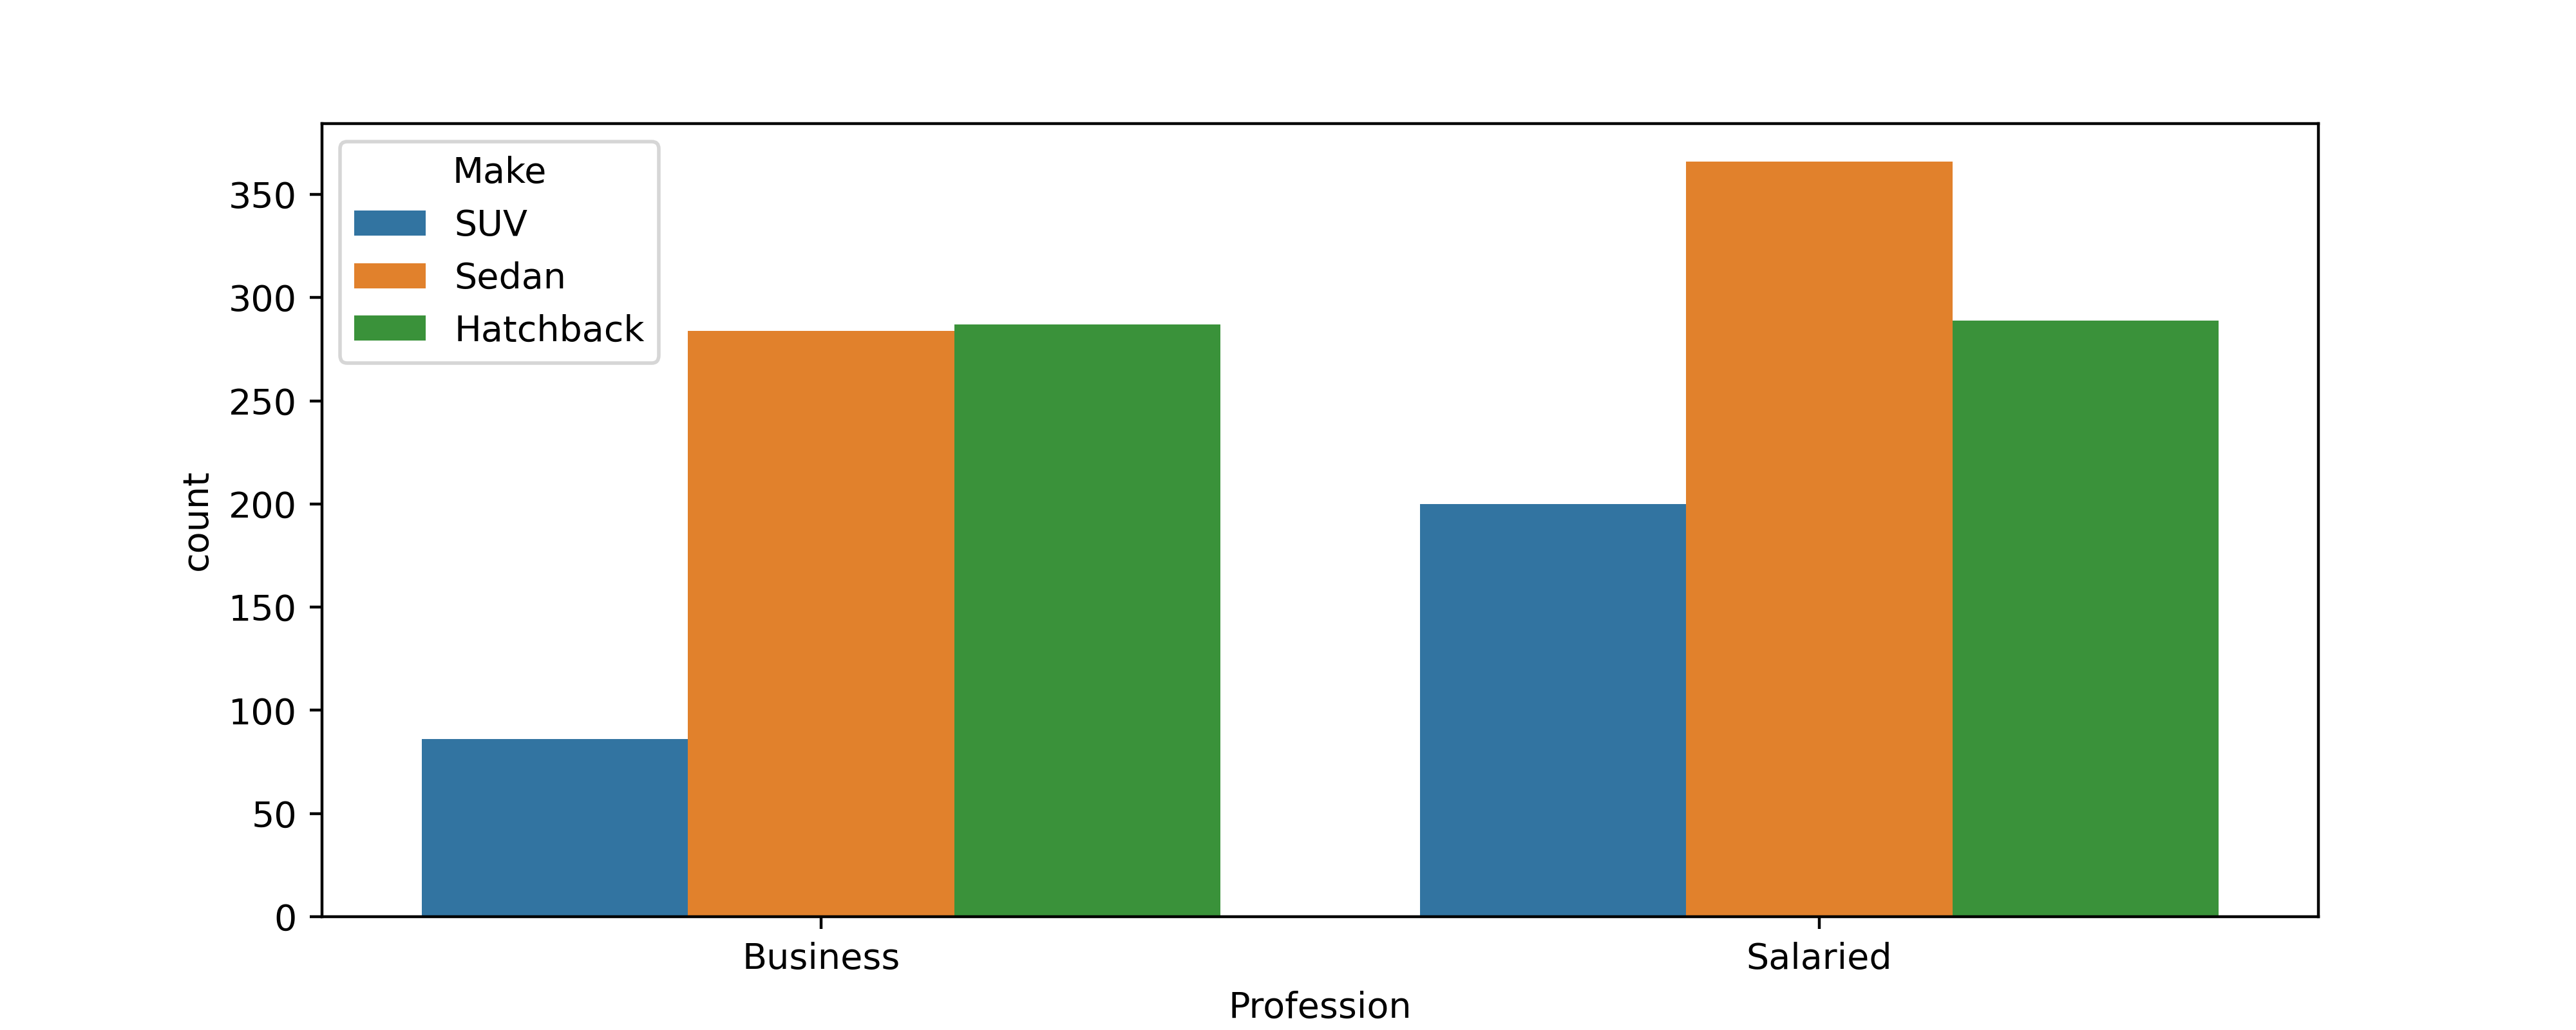
\includegraphics[width=13cm]{make_type_profession.png}
		\caption{Vehicle make preference among salaried and business person.}
	\end{figure}
	
    \subsection{Sheldon Cooper's claim}
    What evidence or data supports Sheldon Cooper's claim that a salaried male is an easier target for a SUV sale over a Sedan sale? For this question we look at preference of make type among salaried men and women. 
    \begin{figure}[h]
    	\centering
    	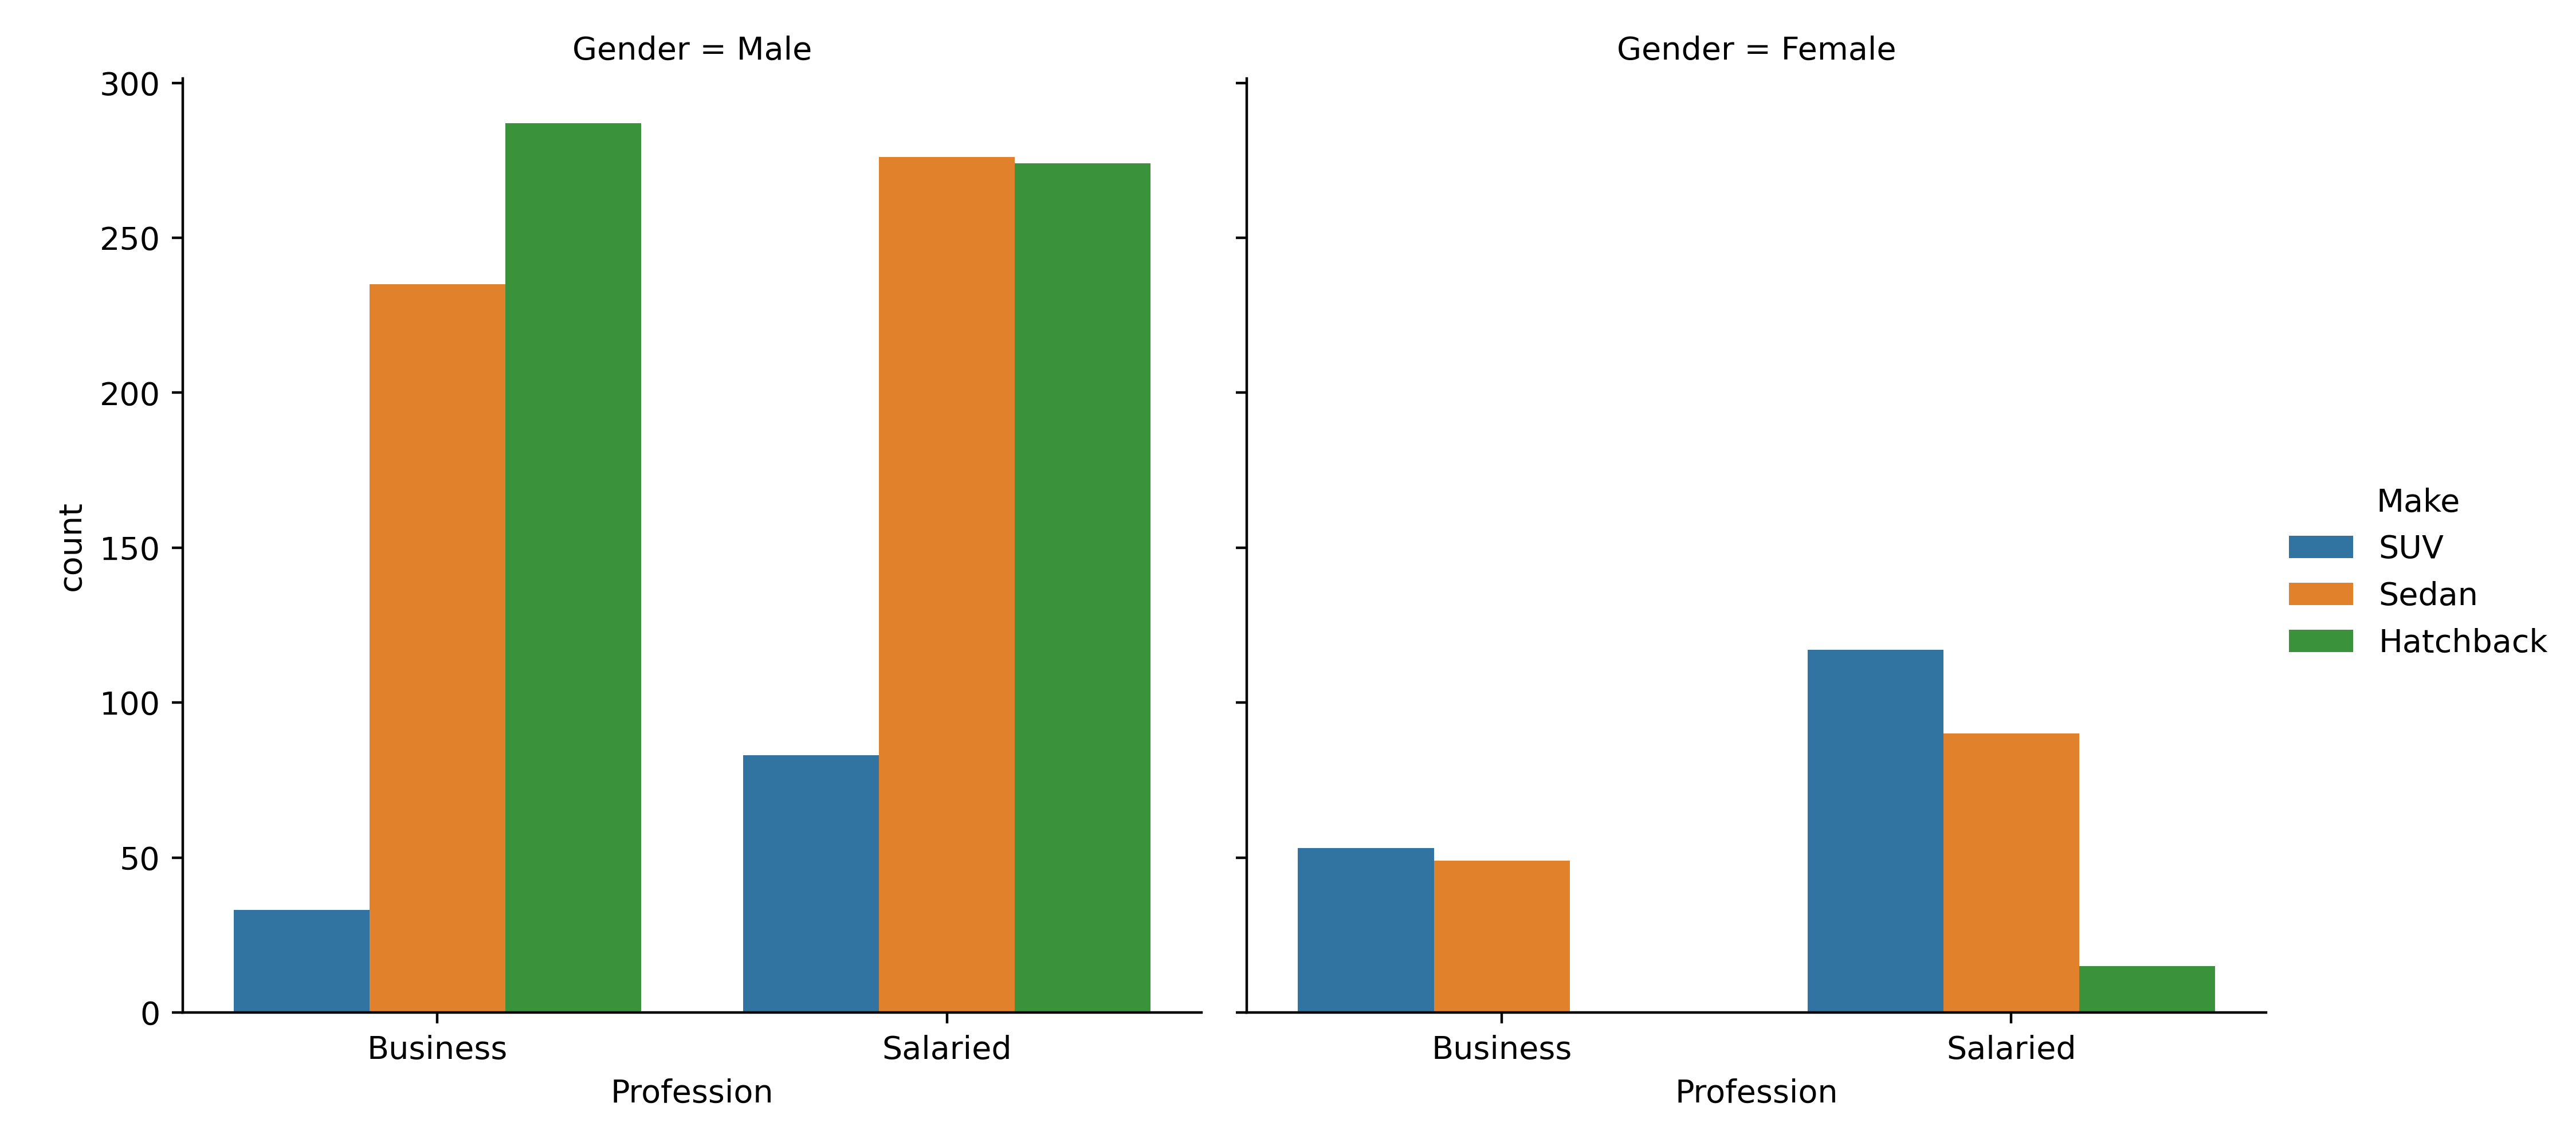
\includegraphics[width=\linewidth]{make_gender_prof_catplot.png}
    	\caption{Vehicle make preference across gender and profession.}
    \end{figure}
    
    \subsection{Variation of amount spent on purchasing automobiles by gender}
    \begin{figure}[h]
    	\centering
    	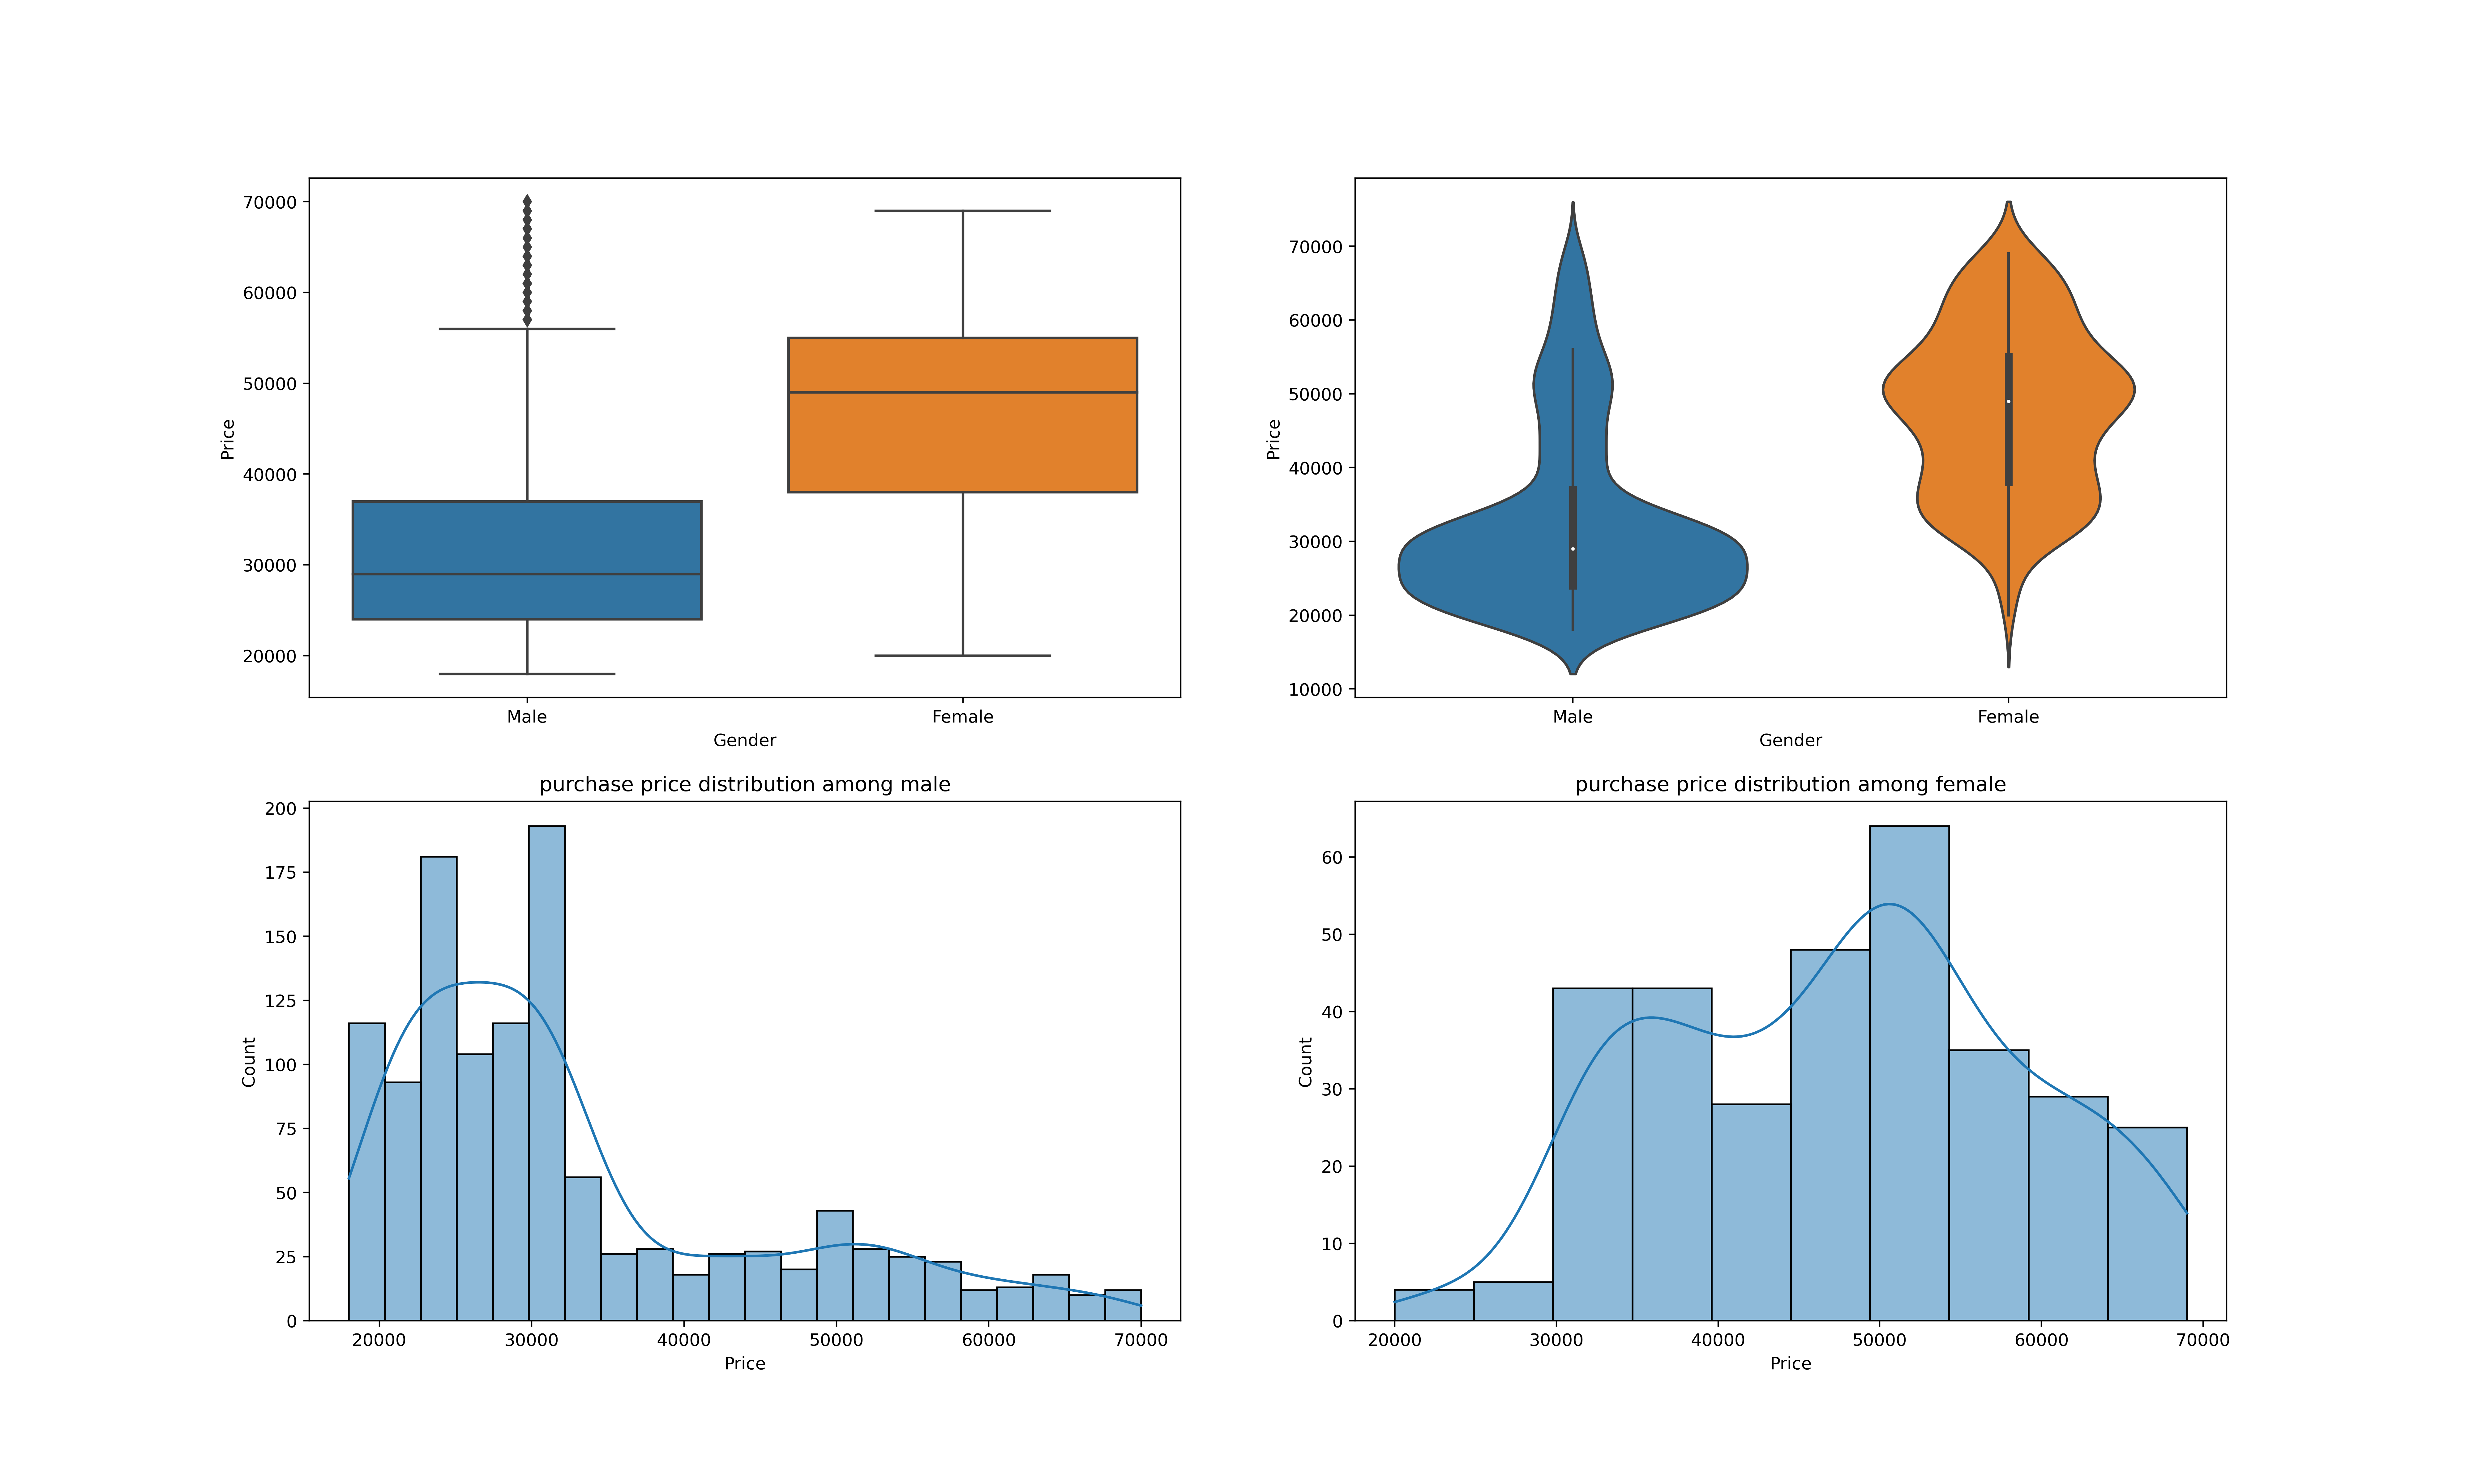
\includegraphics[width=\linewidth]{purchase_gender_dist.png}
    	\caption{Distribution of purchase price among male and female}
    \end{figure}
    
    \subsection{Amount spent by individuals who took a loan}
    	\begin{figure}[h]
    	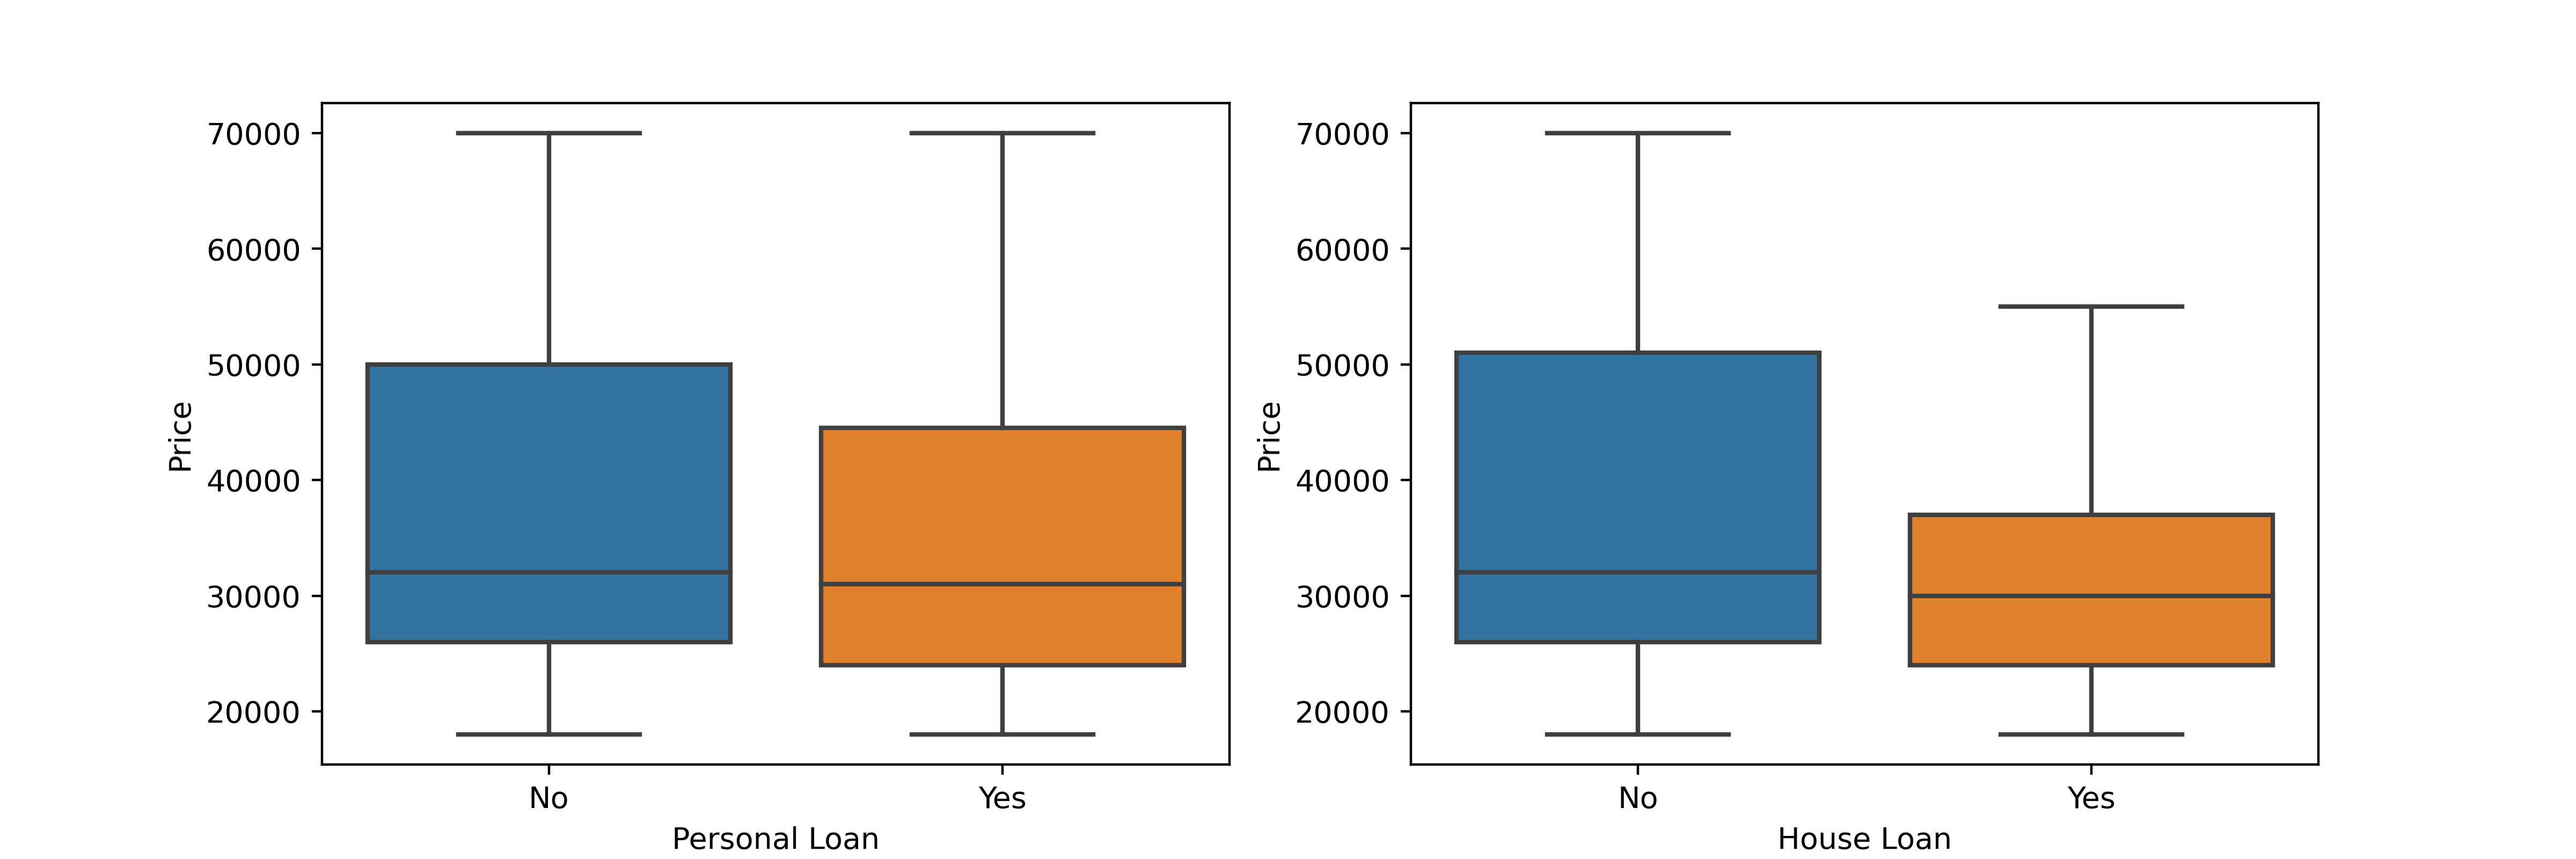
\includegraphics[width=0.8\textwidth]{buyers_with_loan.png}
    	\caption{Amount spent by buyers who have taken loans.}
    	\end{figure}
    
    \subsection{Working partner and purchase of higher priced car}

    	\begin{figure}[h]
    		\centering
			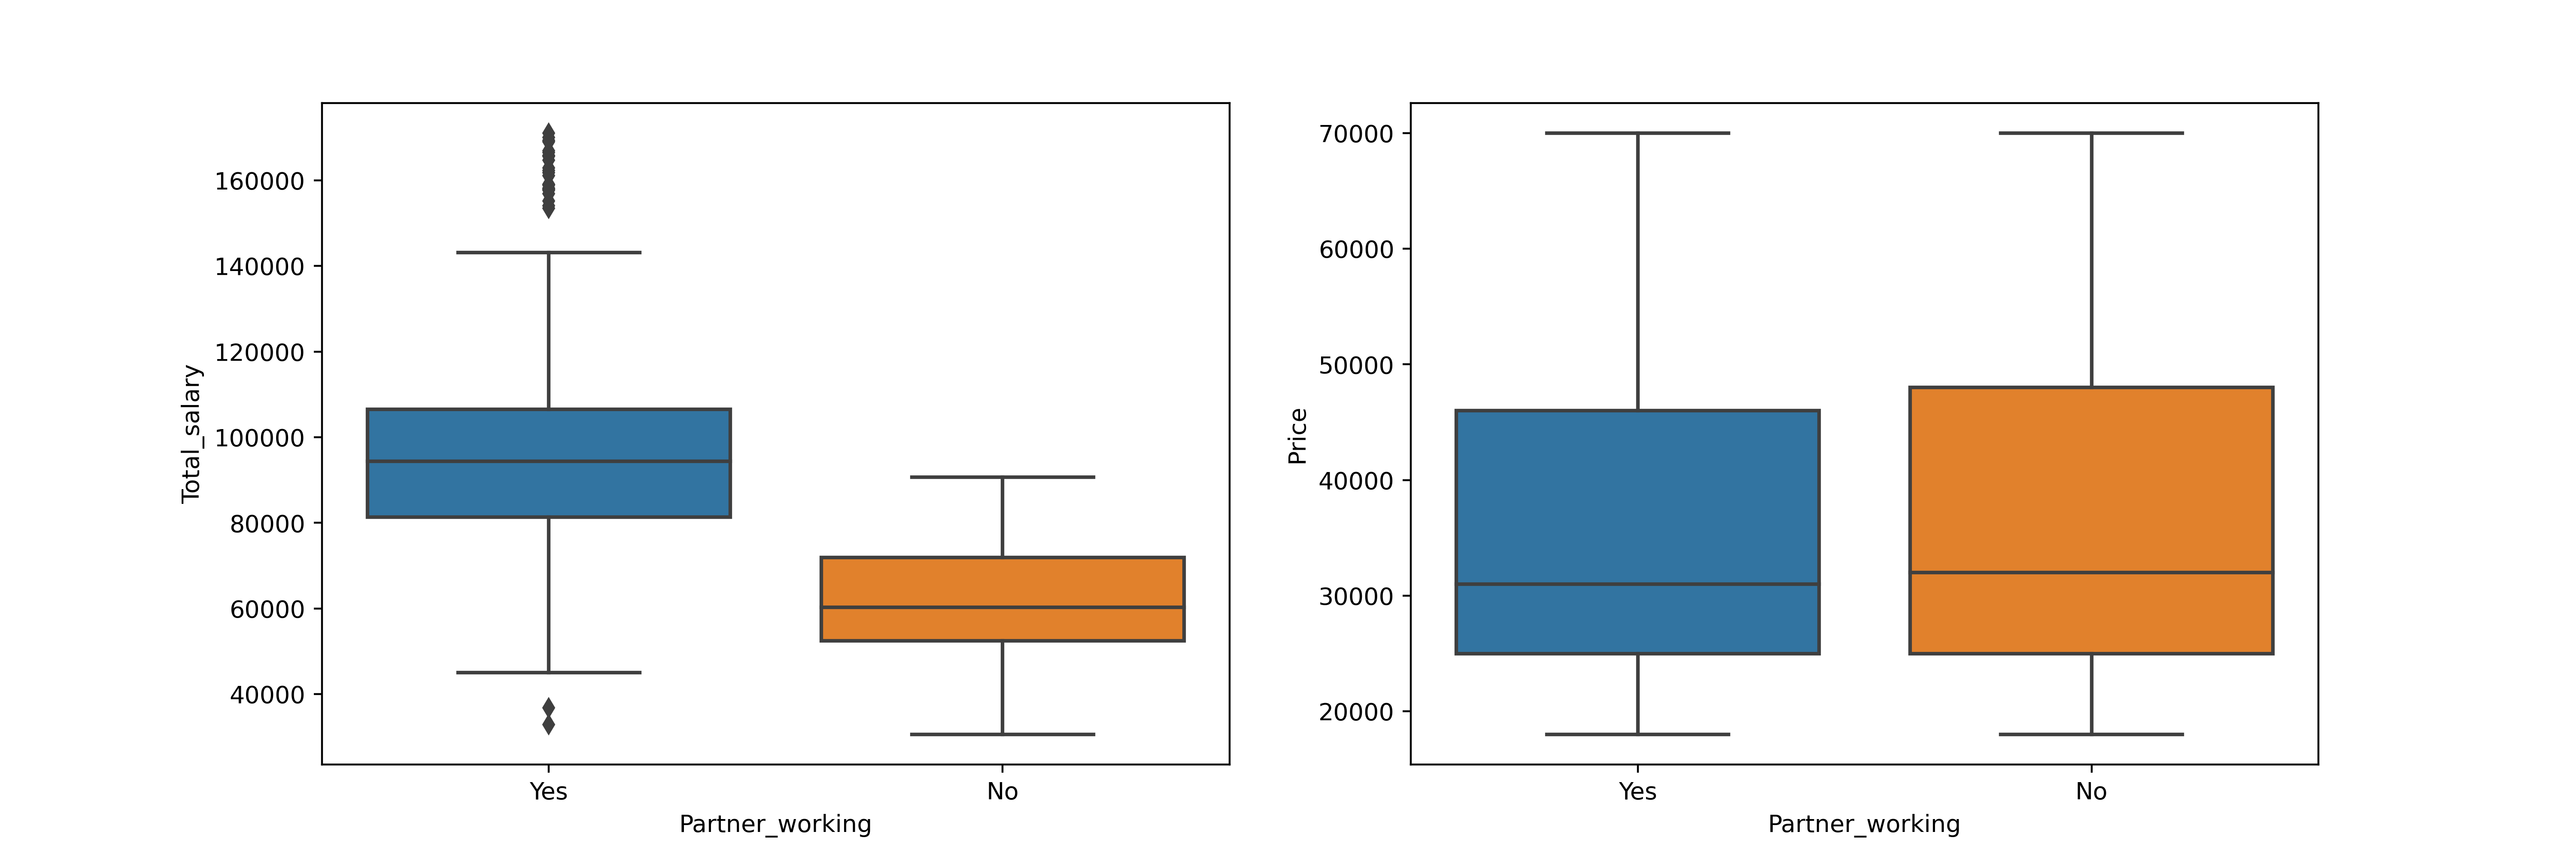
\includegraphics[width=0.9\textwidth]{partner_working_and_price.png}
			\caption{Influence of working partner on purchased price}
		\end{figure}
    %%%%%%%%%%%%%
    \section{Actionable Insights and Recommendations}
    \subsection{Actionable Insights}
    \subsection{Business Recommendations}
    
\end{document}